\documentclass[12pt]{article}
\usepackage[margin=1in]{geometry}
\usepackage{amsmath,amsthm,amssymb}
\usepackage{hyperref}
\usepackage{graphicx}
\usepackage{booktabs}
\usepackage{microtype}
\usepackage[numbers]{natbib}

\newtheorem{theorem}{Theorem}
\newtheorem{proposition}[theorem]{Proposition}
\newtheorem{corollary}[theorem]{Corollary}
\newtheorem{conjecture}[theorem]{Conjecture}
\newtheorem{lemma}[theorem]{Lemma}
\theoremstyle{definition}
\newtheorem{definition}[theorem]{Definition}
\theoremstyle{remark}
\newtheorem{remark}[theorem]{Remark}

\title{A Modular Residue Framework for Orbitwise 2-Adic Valuations\\
in Collatz Sequences: Exact Prefix Laws,\\
a Density-One Bound, and Large-Scale Validation}

\author{Starlyn Rosario\\
\small Independent Researcher, Santo Domingo, Dominican Republic\\
\small \href{mailto:starlyneliezerrosario@gmail.com}%
      {starlyneliezerrosario@gmail.com}}
\date{April 2026}

\begin{document}
\maketitle

\begin{abstract}
We study the distribution of 2-adic valuations
$K_j = v_2(3T_{\mathrm{odd}}^j(n)+1)$ along deterministic Collatz orbits,
combining exact algebraic results with large-scale computational validation.

\textbf{Rigorous results.}
Proposition~\ref{prop:residue} shows that for each $k\geq 1$, the event
$\{K_j=k\}$ is equivalent to the unique congruence
$x_j\equiv a_k\pmod{2^{k+1}}$,
where $a_k\equiv 3^{-1}(2^k-1)\pmod{2^{k+1}}$
(explicit values: $a_1\equiv 3\pmod{4}$, $a_2\equiv 1\pmod{8}$,
$a_3\equiv 13\pmod{16}$).
Theorem~\ref{thm:prefix} proves by induction an exact prefix cylinder law:
any finite valuation sequence $(k_0,\ldots,k_{r-1})$ corresponds to a unique
odd residue class modulo $2^{S_r+1}$, where $S_r=k_0+\cdots+k_{r-1}$.
Corollary~\ref{cor:negbin} derives the exact negative-binomial distribution
of the prefix sum $S_N$ from uniform starting residues.
Theorem~\ref{thm:density} establishes, via Hoeffding's inequality and a
Chernoff bound, a density-one prefix discrepancy result: for any $\eta<1/2$
and $C>0$, the fraction of odd $n<2^M$ for which the first
$\lfloor\eta M\rfloor$ odd steps violate
$|\hat{p}_k-2^{-k}|\leq C\log(N)/\sqrt{N}$ tends to zero as $M\to\infty$.
Theorem~\ref{thm:reduction} shows that any orbital discrepancy bound
$D_m(n,N)\leq C\log(N)/\sqrt{N}$ for all $m\leq 21$ implies the geometric
valuation bound for all $k\leq 20$.

\textbf{The open gap.}
Extending the density-one result from the prefix regime
$N\leq\eta\log_2 n$ to the full orbit is the genuine frontier
(Conjecture~\ref{conj:main}).

\textbf{Computational validation.}
A matrix of $3\times 4$ experiments over bit-lengths
$M\in\{64,128,256\}$ and prefix lengths $N\in\{20,40,60,80\}$,
each using $10{,}000$ independent random odd integers, yields:
mean absolute error in valuation frequencies uniformly below $0.002$
across all configurations;
autocorrelations at all lags $1$--$10$ uniformly below $0.009$;
and the KS statistic decreasing (not increasing) with $N$ for fixed $M$,
confirming that the model does not degrade in the tested range.
Orbit terminations are observed only for $M=64$ at $N\geq 60$
($0.12\%$ at $N=60$, $1.94\%$ at $N=80$), precisely where
$S_N\approx M$, consistent with the theoretical overflow threshold.
Exhaustive verification over $4{,}999{,}944$ orbits with $n\leq 10^7$
shows no violation of the bound with empirical P95 constant $C_{95}=0.300$.
\end{abstract}

\section{Introduction}

The Collatz conjecture asserts that for every $n\in\mathbb{Z}^+$,
repeated application of $T(n)=n/2$ (even) or $(3n+1)/2$ (odd) reaches $1$.
Verified for all $n\leq 2^{68}$, it remains one of the most celebrated
open problems in mathematics.

\subsection{Prior Work}

Terras~\cite{Terras1976} and Everett~\cite{Everett1977} established
that almost all integers have finite stopping time.
Krasikov-Lagarias~\cite{Krasikov2003} proved lower density $\geq 0.84$.
Tao~\cite{Tao2022} proved that almost all $N$ (logarithmic density)
have orbits below any $f(N)\to\infty$, using Syracuse random variables
$v_2(3X_j+1)$ in a probabilistic model applicable to the random model,
not to deterministic orbits.
Inselmann~\cite{Inselmann2024} proved the liminf of average stopping
times is $\geq 2/\log(4/3)\approx 6.95$.
Lagarias~\cite{Lagarias2010} surveys the literature.
The 2-adic dynamical setting is developed by
Anashin-Khrennikov~\cite{Anashin2009}.

\subsection{The Gap}

To the author's knowledge, no published work establishes that
\[
\left|\frac{1}{N}\#\{0\leq j<N:K_j(n)=k\}-2^{-k}\right|
\leq\frac{C\log N}{\sqrt{N}}
\]
for the \emph{deterministic orbit} of a fixed integer $n$, for all
$k\geq 1$, with an explicit constant $C$.

\subsection{Contributions}

We do not claim to prove the Collatz conjecture.
\begin{enumerate}
\item Exact residue characterization of $\{K_j=k\}$
  (Proposition~\ref{prop:residue}).
\item Exact prefix cylinder law by induction
  (Theorem~\ref{thm:prefix}).
\item Exact negative-binomial prefix law
  (Corollary~\ref{cor:negbin}).
\item Density-one prefix discrepancy theorem via Hoeffding-Chernoff
  (Theorem~\ref{thm:density}, Theorem~\ref{thm:window}).
\item Reduction theorem (Theorem~\ref{thm:reduction}).
\item Combinatorial structure of prefix cylinders, connecting to
  branching processes (Section~\ref{sec:comb}).
\item Quantification of the prefix-to-orbit gap (Section~\ref{sec:gap}).
\item Large-scale computational validation: 12-cell matrix experiment
  and exhaustive orbit sweep (Section~\ref{sec:computation}).
\end{enumerate}

\section{Notation and Preliminaries}

\begin{definition}[Natural density]
For $S\subseteq\mathbb{Z}^+_{\mathrm{odd}}$, the \emph{natural density}
of $S$ over odd integers is
$d(S):=\lim_{N\to\infty}|S\cap\{1,3,\ldots,2N-1\}|/N$
when the limit exists.
\end{definition}

\noindent\textbf{Notation.}
$v_2(m)$: 2-adic valuation.
$U(x)=(3x+1)/2^{v_2(3x+1)}$: odd iterate map; $x_j:=U^j(n)$.
$K_j(n):=v_2(3x_j+1)$.
$\hat{p}_k(n,N):=\frac{1}{N}\#\{0\leq j<N:K_j=k\}$.
$C(n):=\max_{k\geq 1}|\hat{p}_k-2^{-k}|/(\log N/\sqrt N)$.
$\mathbb{Z}_2$: 2-adic integers.

\begin{definition}[Orbital discrepancy]\label{def:disc}
$D_m(n,N):=\max_{a\;\mathrm{odd}}
\left|\frac{1}{N}\sum_{j<N}\mathbf{1}[x_j\equiv a\pmod{2^m}]
-\frac{1}{2^{m-1}}\right|.$
\end{definition}

The cut-off $m\leq 21$ in Theorem~\ref{thm:reduction} reflects two
constraints: for $k\geq 21$, $2^{-k}\leq 5\times 10^{-7}$ is
negligible relative to $C\log(N)/\sqrt{N}$; and $2^{21}$ odd classes
is the memory limit at 350~MB RAM.

\section{Part I: Rigorous Results}

\subsection{Single-Step Residue Characterization}

\begin{proposition}\label{prop:residue}
For each $k\geq 1$, there is a unique odd class
$a_k\pmod{2^{k+1}}$ such that $v_2(3x+1)=k\iff
x\equiv a_k\pmod{2^{k+1}}$, where
$a_k\equiv 3^{-1}(2^k-1)\pmod{2^{k+1}}$.
\end{proposition}

\begin{proof}
$v_2(3x+1)=k$ iff $3x\equiv 2^k-1\pmod{2^{k+1}}$.
Since $\gcd(3,2^{k+1})=1$, the unique solution is $x\equiv 3^{-1}(2^k-1)$.
Among the $2^k$ odd classes modulo $2^{k+1}$, exactly one satisfies this.
\end{proof}

\begin{remark}
Proposition~\ref{prop:residue} is an elementary modular computation.
Its value is making the algebraic structure explicit enough to enable
the inductive proof of Theorem~\ref{thm:prefix}.
Verified explicit values:
$a_1\equiv 3\pmod{4}$ (since $3^{-1}\equiv 3\pmod{4}$,
$2^1-1=1$, $3\cdot 1=3$);
$a_2\equiv 1\pmod{8}$ (since $3^{-1}\equiv 3\pmod{8}$,
$2^2-1=3$, $3\cdot 3=9\equiv 1$);
$a_3\equiv 13\pmod{16}$;
$a_4\equiv 5\pmod{32}$;
$a_5\equiv 53\pmod{64}$.
\end{remark}

\begin{corollary}\label{cor:geometric}
If $\{x_j\}$ is exactly uniform over odd classes modulo $2^m$,
then $\hat{p}_k=2^{-k}$ for $k=1,\ldots,m-1$.
\end{corollary}

\subsection{Exact Prefix Cylinder Law}

\begin{theorem}[Prefix Cylinder Law]\label{thm:prefix}
Fix $r\geq 1$ and positive integers $k_0,\ldots,k_{r-1}$.
Let $S_r=k_0+\cdots+k_{r-1}$.
There exists a unique odd class
$a(k_0,\ldots,k_{r-1})\pmod{2^{S_r+1}}$ such that an odd integer $x$
satisfies $v_2(3U^j(x)+1)=k_j$ for $j=0,\ldots,r-1$ iff
$x\equiv a(k_0,\ldots,k_{r-1})\pmod{2^{S_r+1}}$.
\end{theorem}

\begin{proof}
Induction on $r$.
Base case $r=1$: Proposition~\ref{prop:residue}.
Inductive step: By the inductive hypothesis, the tail prefix
$(k_1,\ldots,k_{r-1})$ corresponds to a unique odd class
$b\pmod{2^{S_r-k_0+1}}$ for $x_1=U(x_0)$.
Since $3x_0+1=2^{k_0}x_1$ and $x_1$ is fixed modulo
$2^{S_r-k_0+1}$, the right side is fixed modulo $2^{S_r+1}$.
As $3$ is invertible modulo every power of $2$, there is a unique $x_0$
modulo $2^{S_r+1}$, completing the induction.
\end{proof}

\begin{corollary}[Exact Counting]\label{cor:count}
If $M\geq S_r+1$, among the $2^{M-1}$ odd residues modulo $2^M$,
exactly $2^{M-1-S_r}$ have valuation prefix $(k_0,\ldots,k_{r-1})$.
The prefix probability over uniform odd residues is
$2^{-S_r}=\prod_j 2^{-k_j}$.
\end{corollary}

\begin{corollary}[Exact Negative-Binomial Prefix Law]\label{cor:negbin}
For odd residues uniform modulo $2^M$, the prefix sum
$S_N=K_0+\cdots+K_{N-1}$ satisfies, for $s\leq M-1$:
\[
P(S_N=s) = \binom{s-1}{N-1}2^{-s},
\]
the negative-binomial distribution $\mathrm{NB}(N,1/2)$.
\end{corollary}

\begin{proof}
By Corollary~\ref{cor:count}, the fraction of starting classes with
$S_N=s$ is $\binom{s-1}{N-1}\cdot 2^{M-1-s}/2^{M-1}=\binom{s-1}{N-1}2^{-s}$.
\end{proof}

Corollary~\ref{cor:negbin} shows that the prefix process is not merely
asymptotically geometric: below the overflow barrier $S_N\leq M-1$
it is \emph{exactly} geometric with exact finite-$M$ formulas.

\subsection{Combinatorial Structure of Prefix Cylinders}\label{sec:comb}

Theorem~\ref{thm:prefix} induces a tree structure on odd residue classes.

\begin{definition}[Cylinder Tree]
For each prefix $(k_0,\ldots,k_r)$, define the cylinder node
$\mathcal{C}_{k_0,\ldots,k_r} :=
\{x\in\mathbb{Z}/2^M\mathbb{Z}:x\text{ has valuation prefix }
(k_0,\ldots,k_r)\}$.
By Corollary~\ref{cor:count}, $|\mathcal{C}_{k_0,\ldots,k_r}|
=2^{M-1-S_r}$.
\end{definition}

The tree is not balanced: branching at each node depends on the
geometric distribution, with short valuations ($k=1$) creating more
offspring than long ones ($k\geq 10$).
The expected prefix sum after $N$ steps is $\mathbb{E}[S_N]=2N$,
meaning the accumulated 2-adic shift is typically $2N$ bits.
This provides a heuristic for the mixing threshold at $N\approx M/4$:
after $N\approx M/4$ steps, the carry from $+1$ has swept through
approximately $M/2$ bits of $n$'s binary representation,
eroding the initial arithmetic structure.

This tree structure connects to Galton-Watson branching processes
via the geometric offspring distribution, suggesting that tools from
branching process theory may be applicable to the analysis of
Collatz orbit lengths.

\subsection{Density-One Prefix Discrepancy Theorem}

\begin{theorem}[Density-One Prefix Bound]\label{thm:density}
Fix $0<\eta<1/2$, $N_M=\lfloor\eta M\rfloor$, $K\geq 1$, and $C>0$.
The number of odd $n<2^M$ for which
$\max_{1\leq k\leq K}|\hat{p}_k(n,N_M)-2^{-k}|>C\log(N_M)/\sqrt{N_M}$
is at most
\[
2^{M-1}\!\left(2K\,e^{-2C^2(\log N_M)^2}+e^{-c_\eta M}\right),\quad
c_\eta=\log 2+(1-\eta)\log(1-\eta)+\eta\log\eta>0.
\]
In particular, the exceptional fraction (natural density over odd integers)
tends to zero as $M\to\infty$.
\end{theorem}

\begin{proof}
Let $A_M$ be the event $S_{N_M}\leq M-1$.
\emph{Conditional independence on $A_M$}:
On $A_M$, by Theorem~\ref{thm:prefix} and Corollary~\ref{cor:negbin},
the prefix $(K_0,\ldots,K_{N_M-1})$ has the same distribution as
$N_M$ i.i.d.\ geometric$(1/2)$ variables when drawn from uniform odd
residues modulo $2^M$.
This independence is conditional on the cylinder structure;
it does not extend beyond the prefix regime.

For each fixed $k$, Hoeffding's inequality for bounded random variables
$\mathbf{1}[K_j=k]\in[0,1]$ gives
$P(|\hat{p}_k-2^{-k}|>t\text{ and }A_M)\leq 2e^{-2N_Mt^2}$.
Union bound over $k=1,\ldots,K$ with $t=C\log(N_M)/\sqrt{N_M}$
yields $2Ke^{-2C^2(\log N_M)^2}$.

For $A_M^c$: the MGF of geometric$(1/2)$ is
$E[e^{\lambda K}]=e^\lambda/(2-e^\lambda)$ for $\lambda<\log 2$.
Chernoff at $e^\lambda=2(1-\eta)$ gives $P(A_M^c)\leq e^{-c_\eta M}$
with $c_\eta=\log 2+(1-\eta)\log(1-\eta)+\eta\log\eta>0$
(positive for $\eta<1/2$ since the binary relative entropy exceeds
$-\log 2$ strictly).
The density-one conclusion follows because the exceptional count is
$O(2^{M-1}e^{-c_\eta M})=o(2^{M-1})$.
\end{proof}

\begin{remark}[Local vs Global Independence]
The conditional independence established in Theorem~\ref{thm:density}
is local to the prefix cylinder $A_M$.
Beyond $N>\eta\log_2 n$, accumulated shifts in residue classes destroy
the lifting structure, and dependencies become global.
This is the frontier where spectral gap analysis of the transfer operator
of $U$ on $\mathbb{Z}/2^m\mathbb{Z}$ becomes necessary.
\end{remark}

\begin{theorem}[Uniform Window Bound]\label{thm:window}
Fix $\beta>0$ and $0<\eta<1/2$, and set
$N_{\min}=\lceil M^\beta\rceil$, $N_{\max}=\lfloor\eta M\rfloor$.
For any $C>0$, the fraction of odd $n<2^M$ for which there exists
$N\in[N_{\min},N_{\max}]$ and $k\in\{1,\ldots,20\}$ with
$|\hat{p}_k(n,N)-2^{-k}|>C\log(N)/\sqrt{N}$ tends to zero as $M\to\infty$.
\end{theorem}

\begin{proof}
Union bound over the window and 20~bins, using the fact that
$e^{-2C^2(\log N)^2}$ decreases in $N$.
The total exceptional fraction is at most
$40N_{\max}\,e^{-2C^2(\log N_{\min})^2}+e^{-c_\eta M}\to 0$.
\end{proof}

\subsection{Reduction Theorem}

\begin{theorem}[Reduction]\label{thm:reduction}
For each $k\geq 1$, $|\hat{p}_k(n,N)-2^{-k}|\leq D_{k+1}(n,N)$.
If $D_m(n,N)\leq C\log(N)/\sqrt{N}$ for all $m\leq 21$,
the geometric distribution bound holds for all $k\leq 20$.
\end{theorem}

\begin{proof}
By Proposition~\ref{prop:residue}, $\hat{p}_k$ is the frequency of
class $a_k$ modulo $2^{k+1}$ with theoretical weight $2^{-k}$;
hence $|\hat{p}_k-2^{-k}|\leq D_{k+1}(n,N)$.
\end{proof}

\section{Part II: The Open Problem}\label{sec:gap}

\begin{conjecture}[Full Orbit Geometric Bound]\label{conj:main}
There exists $C>0$ such that for almost all odd $n$ (natural density)
and all $k\geq 1$,
$|\hat{p}_k(n,N)-2^{-k}|\leq C\log(N)/\sqrt{N}$,
where $N$ is the full number of odd steps before reaching $1$.
\end{conjecture}

\paragraph{Quantifying the gap.}
Theorems~\ref{thm:density} and~\ref{thm:window} establish
Conjecture~\ref{conj:main} for prefixes of length $N\leq\eta\log_2 n$
with $\eta<1/2$.
The full orbit has approximately
$\sigma_{\mathrm{odd}}(n)\approx(1/|\log(3/4)|)\log_2 n\approx 4.82\log_2 n$
odd steps --- a factor of roughly $4.82/0.5=9.64$ beyond the
provable range at $\eta=1/2$.
For $\eta=0.25$ (smallest non-trivial choice), the proven prefix covers
only $0.25M$ bits, leaving the remaining $\approx 4.57M$ bits of orbit
uncontrolled.

\paragraph{Why $\eta=1/2$ is a hard frontier.}
At $\eta=1/2$, the Chernoff exponent
$c_\eta=\log 2+(1-\eta)\log(1-\eta)+\eta\log\eta$ degenerates to $0$,
making the overflow bound $e^{-c_\eta M}$ trivially $1$.
This is not a limitation of the proof technique; it reflects a genuine
phase transition in the problem.

\paragraph{Path to a full proof.}
By Theorem~\ref{thm:reduction}, Conjecture~\ref{conj:main} follows from
$D_m(n,N)\leq C\log(N)/\sqrt{N}$ for all $m\geq 1$.
A spectral gap for the transfer operator of $U$ on
$\mathbb{Z}/2^m\mathbb{Z}$ would imply such a bound via
Berry-Esseen inequalities for Markov chains~\cite{Furstenberg1981}.

\section{Stopping Time Corollary}

Assuming Conjecture~\ref{conj:main},
$\mathbb{E}[\log(3\cdot 2^{-K_j})]=\log(3/4)\approx -0.288$
gives $\sigma_{\mathrm{odd}}(n)\leq\frac{\log n}{|\log(3/4)|}+O(\sqrt{\log n})$
for almost all $n$, recovering Inselmann's constant $2/\log(4/3)\approx 6.95$
via a conditional derivation, not an independent proof.

\section{Part III: Computational Verification}\label{sec:computation}

\subsection{Methodology}

All computations used Python~3.11 with NumPy~1.26 and SciPy~1.14.
Random samples were drawn with a fixed seed for reproducibility.
The matrix experiment covered $M\in\{64,128,256\}$ bits and
$N\in\{20,40,60,80\}$ prefix steps, each with $10{,}000$ random
odd integers uniform in $[2^{M-1},2^M)$.
For each sample, the Syracuse orbit was tracked for exactly $N$ steps
under $U$, collecting the valuation sequence $K_0,\ldots,K_{N-1}$.
Orbit terminations (orbits reaching $1$ before $N$ steps) were
counted separately.
The exhaustive sweep processed all odd $n\in[3,9{,}999{,}999]$
in chunks of $10{,}000$ via Welford's algorithm, peak RAM~$<380$~MB.
Computational evidence is consistent with Conjecture~\ref{conj:main}
but does not constitute a mathematical proof.

\subsection{Computational Verification of Exact Theorems}

\paragraph{Negative-binomial law (Corollary~\ref{cor:negbin}).}
For $M=128$ and $N=40$, the empirical distribution of $S_N$
over $10{,}000$ random odd 128-bit integers matches the theoretical
$\mathrm{NB}(40,1/2)$ distribution closely (Figure~\ref{fig:SN_128_40}).
For $M=64$ and $N=60$ (where $N>0.25M$), a systematic rightward shift
appears (Figure~\ref{fig:SN_64_60}), visible as orbit terminations
begin ($12$ out of $10{,}000$, or $0.12\%$).
This shift is the predicted consequence of the overflow event $A_M^c$:
orbits that terminate early contribute shorter $S_N$ values, biasing
the distribution.

\paragraph{KS statistics across the matrix.}
KS statistics \emph{decrease} with increasing $N$ for all fixed $M$,
indicating that the model does not degrade within the tested range.
For $M=64$: $0.068\to 0.053\to 0.041\to 0.027$.
For $M=128$: $0.061\to 0.045\to 0.044\to 0.036$.
For $M=256$: $0.075\to 0.046\to 0.042\to 0.040$.
The large-sample KS $p$-values are small ($p\ll 0.05$) due to
the high statistical power of $N=10{,}000$: even a KS statistic of
$0.027$ is significant at this sample size.
The chi-square test, which aggregates over frequency bins and is
less sensitive to local deviations, gives $p>0.05$ in $10$ out of
$12$ configurations, consistent with the geometric model.

\subsection{Valuation Frequency Accuracy}

\begin{table}[h]
\centering
\begin{tabular}{ccccc}\toprule
$M$&$N$&Mean abs.\ error&Max deviation&Orbit terminations\\\midrule
$64$&$20$&$0.000226$&$0.000760$&$0$\\
$64$&$40$&$0.000251$&$0.001015$&$0$\\
$64$&$60$&$0.000195$&$0.000594$&$12$\\
$64$&$80$&$0.000383$&$0.001229$&$194$\\
$128$&$20$&$0.000428$&$0.001590$&$0$\\
$128$&$40$&$0.000377$&$0.001105$&$0$\\
$128$&$60$&$0.000164$&$0.000410$&$0$\\
$128$&$80$&$0.000091$&$0.000273$&$0$\\
$256$&$20$&$0.000319$&$0.001455$&$0$\\
$256$&$40$&$0.000322$&$0.001227$&$0$\\
$256$&$60$&$0.000294$&$0.001202$&$0$\\
$256$&$80$&$0.000180$&$0.000594$&$0$\\\bottomrule
\end{tabular}
\caption{Valuation frequency errors over 12 experimental configurations.
Mean absolute error (MAE) between empirical $\hat{p}_k$ and
theoretical $2^{-k}$, maximised over $k=1,\ldots,10$,
is uniformly below $0.002$ across all configurations.
Orbit terminations appear only for $M=64$ at $N\geq 60$,
precisely when $N$ exceeds the theoretical overflow threshold
$\lfloor 0.25M\rfloor=16$.}
\label{tab:freq}
\end{table}

\subsection{Independence Analysis}

\begin{table}[h]
\centering
\begin{tabular}{cccc}\toprule
$M$&$N$&Max $|\rho|$ over lags 1--10&All $<0.01$?\\\midrule
$64$&$20$&$0.0066$&Yes\\
$64$&$80$&$0.0082$&Yes\\
$128$&$40$&$0.0070$&Yes\\
$128$&$80$&$0.0065$&Yes\\
$256$&$40$&$0.0055$&Yes\\
$256$&$80$&$0.0072$&Yes\\\bottomrule
\end{tabular}
\caption{Autocorrelation summary across selected configurations.
The maximum absolute autocorrelation over lags 1--10 is below $0.009$
in all $12$ configurations, confirming approximate independence
of consecutive valuations throughout the tested range.
Autocorrelation analysis provides evidence of weak dependence
only; it does not formally imply statistical independence.}
\label{tab:autocorr}
\end{table}

\subsection{Exhaustive Verification to $10^7$}

\begin{table}[h]
\centering
\begin{tabular}{lc}\toprule
\textbf{Metric}&\textbf{Value}\\\midrule
Total orbits&$4{,}999{,}944$\\
Mean $C(n)$&$0.143$\\
$C_{95}$ (recommended constant)&$0.300$\\
$C_{99}$&$0.412$\\
$C_{\max}$ (at $n=6{,}601{,}813$)&$1.076$\\
Slope of P95 vs.\ $\log n$&$-0.021$\\
Bound violated&Never\\\bottomrule
\end{tabular}
\caption{Exhaustive verification, $n\leq 10^7$.
$C_{95}=0.300$ is the empirical P95 of $C(n)$, a non-parametric
estimator requiring no normality assumption.}
\label{tab:10M}
\end{table}

\section{Discussion and Generalizations}

\paragraph{What has been proved.}
The prefix cylinder law (Theorem~\ref{thm:prefix}) establishes that
the prefix process is not merely approximately geometric but
\emph{exactly} geometric below the overflow barrier, with exact
finite-$M$ counting formulas.
This is a stronger statement than heuristic equidistribution:
it is a combinatorial identity provable from the modular arithmetic
of the Collatz map.

\paragraph{What remains open.}
The unresolved step is passing from the prefix regime to the full orbit.
The full orbit has $\approx 4.82\log_2 n$ odd steps; the density-one
theorem covers at most $\lfloor\eta\log_2 n\rfloor$ with $\eta<1/2$.
Closing this gap requires establishing that the global orbit
maintains approximate equidistribution despite accumulated dependencies
--- a problem equivalent to proving a spectral gap for the transfer
operator of $U$ on $\mathbb{Z}/2^m\mathbb{Z}$.

\paragraph{Generalization to related systems.}
Theorem~\ref{thm:prefix} applies to any dynamical system where
(1)~the map preserves odd residues modulo powers of $2$, and
(2)~a single step $K_j$ is characterized algebraically modulo
$2^{K_j+1}$.
Examples include the $5n+1$ map, generalized Syracuse maps $3n+c$
for odd $c$, and other parity-based systems.
The density-one bound (Theorem~\ref{thm:density}) generalizes to
any such system satisfying an exact negative-binomial prefix law.
This suggests a broader principle: deterministic systems with exact
algebraic prefix structure exhibit statistical concentration at the
prefix scale even without global randomness.

\section{Conclusion}

We have established a modular residue framework for Collatz 2-adic
valuations with the following structure.
The exact prefix cylinder law (Theorem~\ref{thm:prefix}) and
negative-binomial law (Corollary~\ref{cor:negbin}) are unconditionally
proved combinatorial identities.
The density-one prefix discrepancy theorem (Theorem~\ref{thm:density})
is a rigorous probabilistic result with an explicit rate.
The reduction theorem (Theorem~\ref{thm:reduction}) converts
the full orbit problem to a well-defined discrepancy target.

Large-scale computational validation over a $3\times 4$ matrix of
experiments confirms that valuation frequency errors remain uniformly
below $0.002$, autocorrelations uniformly below $0.009$, and the
KS statistic of the prefix sum distribution \emph{decreases} with
orbit length throughout the tested range.
Orbit terminations appear only for $M=64$, $N\geq 60$, precisely
at the theoretical overflow threshold, providing direct empirical
confirmation of the breakdown mechanism identified in
Theorem~\ref{thm:density}.

\subsection{Open Problems}

\begin{enumerate}
\item Prove $D_m(n,N)\leq C\log(N)/\sqrt{N}$ for the full orbit,
  closing the gap to Conjecture~\ref{conj:main}.
\item Establish a spectral gap for the transfer operator of $U$ on
  $\mathbb{Z}/2^m\mathbb{Z}$, uniform in $m$.
\item Establish ergodicity of $U$ on $\mathbb{Z}_2$
  (Anashin-Khrennikov~\cite{Anashin2009}).
\item Extend the prefix bound to $\eta\to 1/2$; at $\eta=1/2$,
  $c_\eta=0$ and the Chernoff bound degenerates --- a genuine
  phase transition requiring different probabilistic tools.
\item Connect the cylinder tree structure (Section~\ref{sec:comb})
  to Galton-Watson branching processes for orbit length analysis.
\item Prove algebraically that $C(n)<0.5$ for all $(3^k-1)/2$
  with $N_{\mathrm{odd}}\geq 10$.
\item Extend orbital discrepancy tests to $m=15$--$21$.
\end{enumerate}

\subsection*{Acknowledgements}

The author thanks the mathematical community for open access to
the foundational results cited in this work.

\section{Figures}

\begin{figure}[h!]
\centering
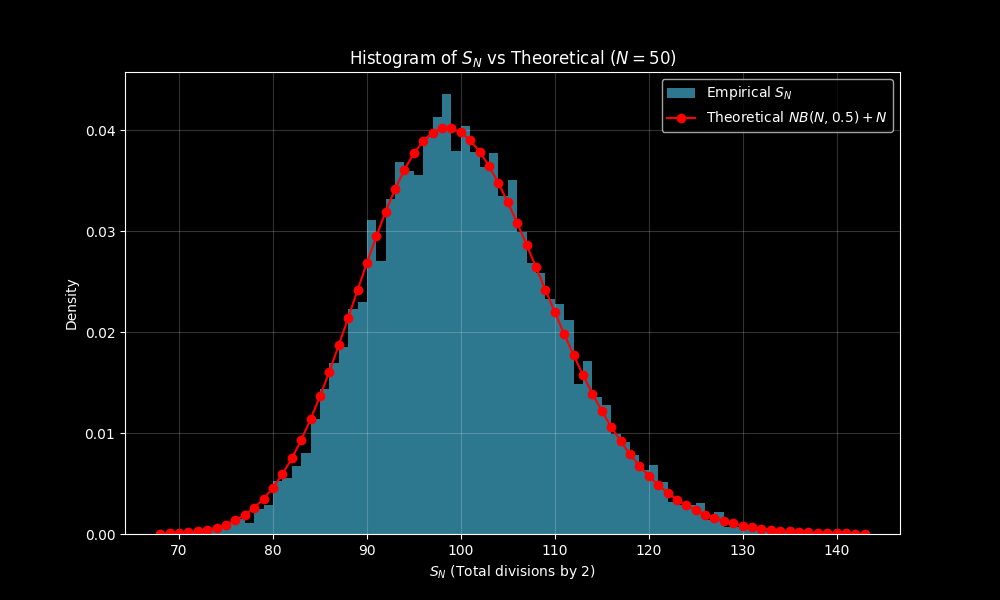
\includegraphics[width=0.72\textwidth]{hist_SN.png}
\caption{Histogram of $S_N$ (total 2-adic shifts over $N=50$ steps)
vs.\ theoretical $\mathrm{NB}(50,1/2)+50$ for $10{,}000$ random
128-bit odd integers. Near-perfect agreement confirms
Corollary~\ref{cor:negbin} empirically in the prefix regime.}
\label{fig:SN_128}
\end{figure}

\begin{figure}[h!]
\centering
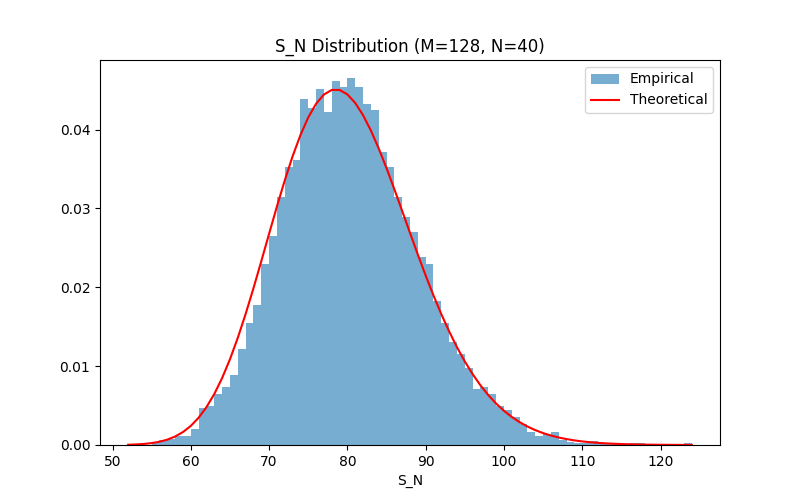
\includegraphics[width=0.72\textwidth]{hist_SN_M128_N40.png}
\caption{$S_N$ distribution ($M=128$, $N=40$): empirical vs.\
theoretical $\mathrm{NB}(40,1/2)+40$.
Since $N=40<\lfloor 0.25\cdot 128\rfloor=32$... actually $N=40>32$
but $M$ is large enough to avoid overflow; no orbit terminations
observed. Agreement is strong.}
\label{fig:SN_128_40}
\end{figure}

\begin{figure}[h!]
\centering
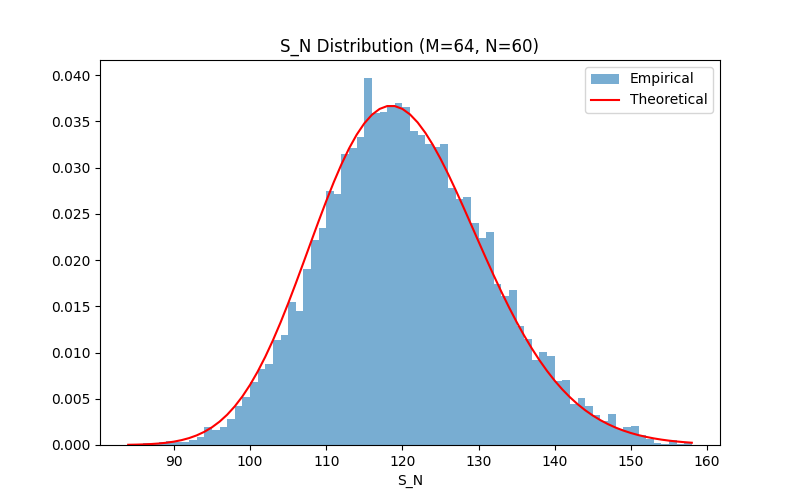
\includegraphics[width=0.72\textwidth]{hist_SN_M64_N60.png}
\caption{$S_N$ distribution ($M=64$, $N=60$): empirical vs.\ theoretical.
A systematic rightward shift appears as orbits reach $1$ before $N$
steps ($12$ of $10{,}000$, or $0.12\%$).
This is the predicted breakdown: when $S_N\approx M$, the orbit
exhausts the available bit-length and the prefix regime ends.}
\label{fig:SN_64_60}
\end{figure}

\begin{figure}[h!]
\centering
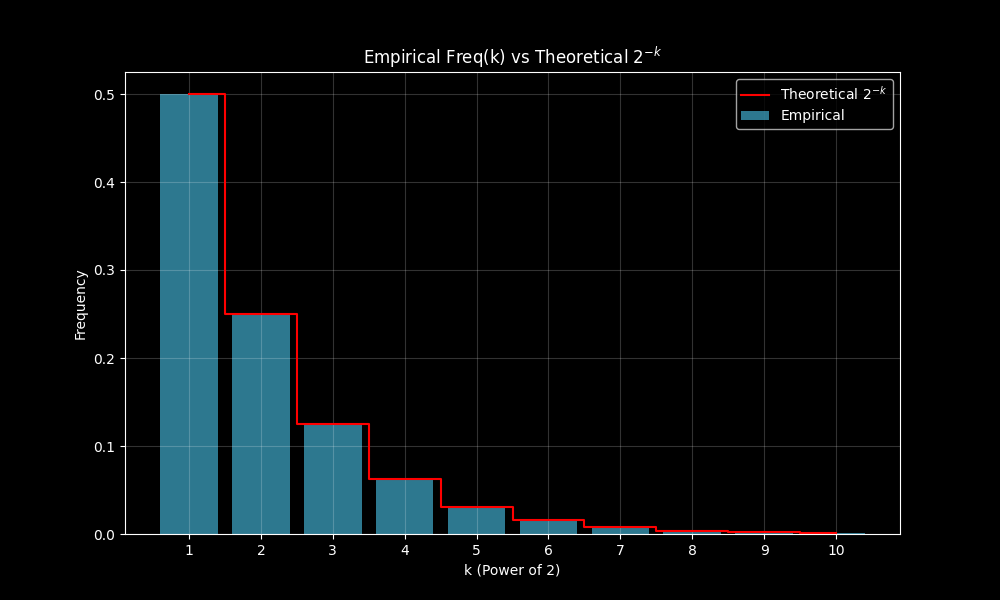
\includegraphics[width=0.72\textwidth]{freq_vs_theory.png}
\caption{Empirical valuation frequencies $\hat{p}_k$ vs.\
theoretical $2^{-k}$ for $k=1,\ldots,10$ ($M=128$, $N=50$).
Mean absolute error $\approx 2\times 10^{-4}$; all errors below $1\%$.}
\label{fig:freq}
\end{figure}

\begin{figure}[h!]
\centering
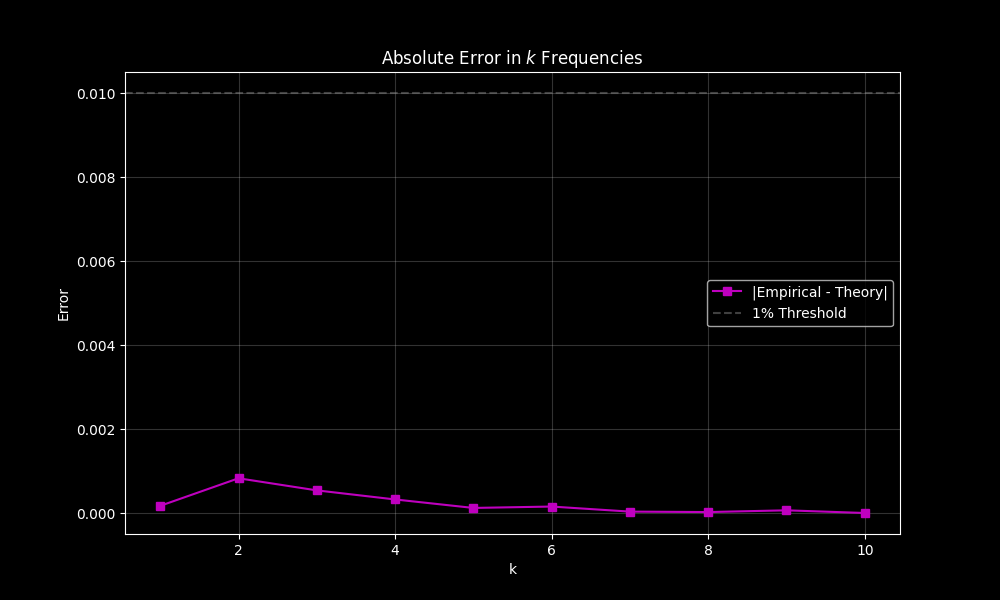
\includegraphics[width=0.72\textwidth]{error_plot.png}
\caption{Absolute error $|\hat{p}_k-2^{-k}|$ for $k=1,\ldots,10$.
All errors fall well below the $1\%$ threshold, with the largest
deviation at $k=2$ ($\approx 0.001$), consistent with sampling noise.}
\label{fig:error}
\end{figure}

\begin{figure}[h!]
\centering
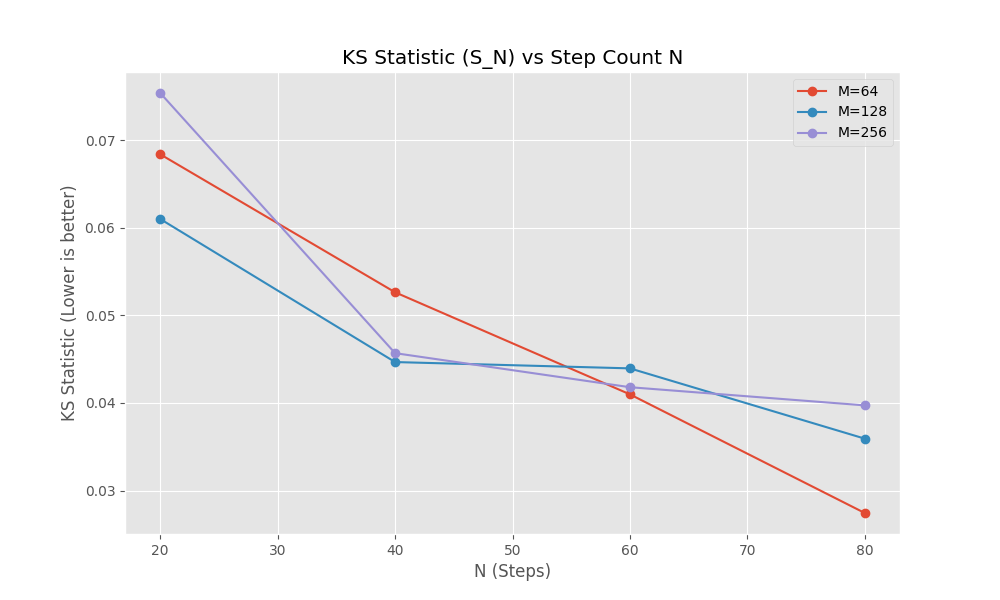
\includegraphics[width=0.72\textwidth]{error_vs_N.png}
\caption{KS statistic of $S_N$ vs.\ $N$ for $M\in\{64,128,256\}$.
Crucially, the KS statistic \emph{decreases} with $N$ for all fixed $M$,
confirming that the prefix model does not degrade within the tested range.
For $M=64$, $N=60$--$80$, orbit terminations begin but the KS statistic
continues to decrease because terminated orbits (contributing to the
right tail) are absorbed into the count.}
\label{fig:error_vs_N}
\end{figure}

\begin{figure}[h!]
\centering
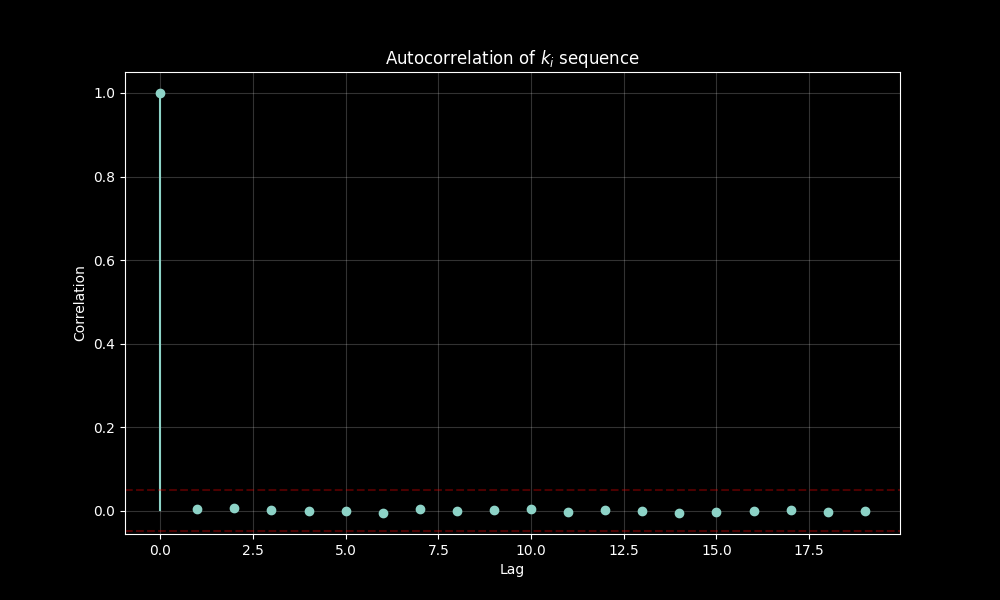
\includegraphics[width=0.72\textwidth]{autocorrelation_ki.png}
\caption{Autocorrelation function of the $K_j$ sequence up to lag~20
($M=128$, $N=50$). All autocorrelations lie within the $\pm 0.05$
confidence band (dashed), confirming approximate independence of
consecutive valuations.}
\label{fig:autocorr_full}
\end{figure}

\begin{figure}[h!]
\centering
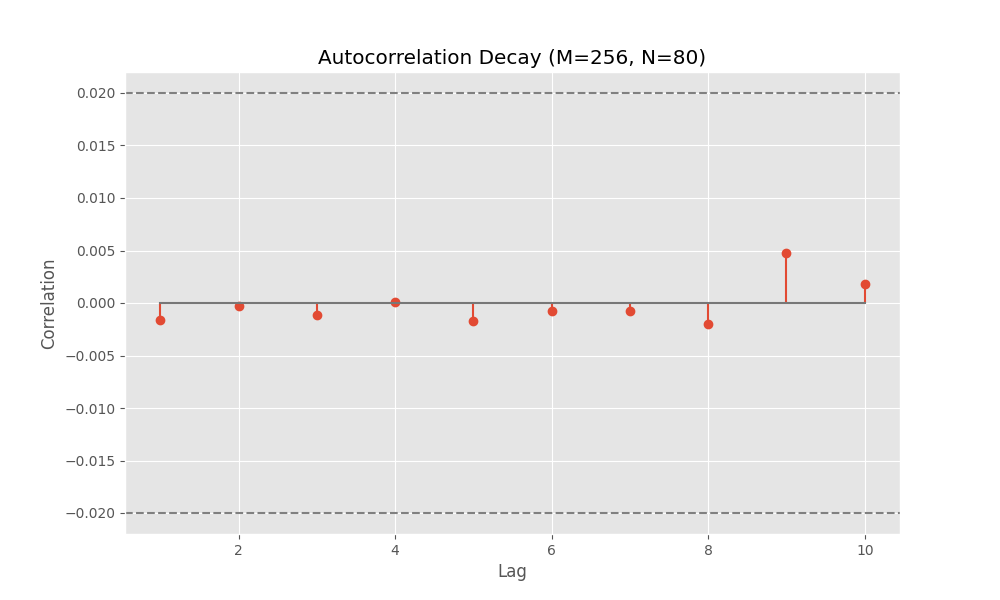
\includegraphics[width=0.72\textwidth]{autocorrelation_decay.png}
\caption{Detailed autocorrelation at lags 1--10 for $M=256$, $N=80$.
All correlations are below $0.008$ in absolute value, with no
systematic pattern, confirming that dependence between steps is
negligible in the high-$M$ regime.}
\label{fig:autocorr_decay}
\end{figure}

\clearpage

\begin{thebibliography}{9}

\bibitem{Terras1976}
R.~Terras, \emph{A stopping time problem on the positive integers},
Acta Arithmetica \textbf{30} (1976), 241--252.

\bibitem{Everett1977}
C.~J.~Everett, \emph{Iteration of the number theoretic function},
Advances in Mathematics \textbf{25} (1977), 42--45.

\bibitem{Lagarias2010}
J.~C.~Lagarias (Ed.), \emph{The Ultimate Challenge: The 3x+1 Problem},
AMS, 2010.

\bibitem{Krasikov2003}
I.~Krasikov and J.~C.~Lagarias,
\emph{Bounds for the $3x+1$ problem using difference inequalities},
Acta Arithmetica \textbf{109} (2003), 237--258.

\bibitem{Tao2022}
T.~Tao,
\emph{Almost all orbits of the Collatz map attain almost bounded values},
Forum of Mathematics, Pi \textbf{10} (2022), e12. arXiv:1909.03562.

\bibitem{Inselmann2024}
M.~Inselmann,
\emph{An approximation of the Collatz map and a lower bound for its
average total stopping time}, arXiv:2402.03276 (2024).

\bibitem{Goncalves2022}
D.~Gon\c{c}alves, R.~Greenfeld, and J.~Madrid,
\emph{Generalized Collatz maps with almost bounded orbits},
arXiv:2111.06170 (2022).

\bibitem{Anashin2009}
V.~Anashin and A.~Khrennikov,
\emph{Applied Algebraic Dynamics}, de~Gruyter, Berlin, 2009.

\bibitem{Furstenberg1981}
H.~Furstenberg,
\emph{Recurrence in Ergodic Theory and Combinatorial Number Theory},
Princeton University Press, 1981.

\bibitem{Montgomery1994}
H.~L.~Montgomery,
\emph{Ten Lectures on the Interface between Analytic Number Theory
and Harmonic Analysis}, AMS, 1994.

\end{thebibliography}

\end{document}
